We present here the expected work plan for this master's thesis. A description of the activities can be found in Section~\ref{sec:Methodology}
\begin{figure}[h]
	\centering
	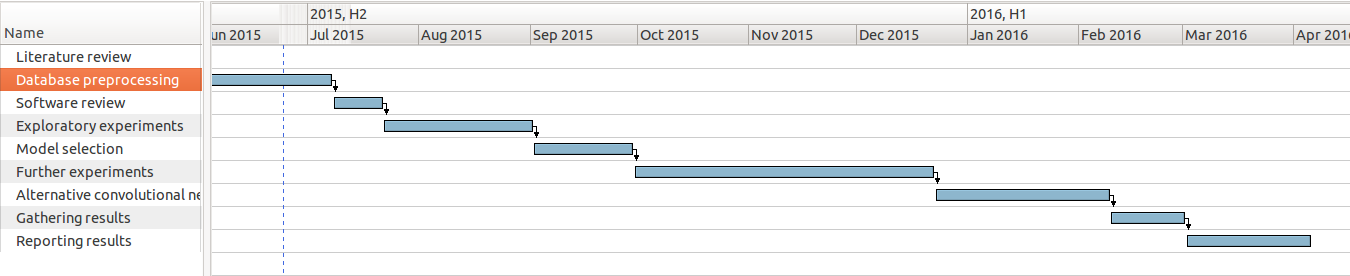
\includegraphics[width = \textwidth]{plots/workplan.png}
	\caption[Thesis Work Plan]{Thesis work plan.}
	\label{fig:workplan}
\end{figure}

Literature and software review and the preprocessing of the image database are expected to be done before the end of the summer term (late July). The first experiments on simple convolutional networks and applicability to breast cancer are expected for the fall semester (late October to early November). At this point, these results should be reported in the thesis and hopefully a scientific article. Later, the final architecture and methods will be selected and the final experiments run. The thesis document should be delivered by the start of March. During this month, if the new results are valuable, we expect to write a conference or journal article to share our results with the community.
\begin{comment}
Una vez establecida la {\it Metodología} es importante establecer las
actividades con sus tiempos respectivos en lo que se llama el {\it Plan de
Trabajo}. Ello nos da una idea clara de la extensión en tiempo del trabajo
propuesto. Además de ser necesario, lo cual es normalmente cierto en
propuestas de proyecto industrial, es importante establecer el PLAN FINANCIERO
el cual desglosa los recursos necesarios para el desarrollo del proyecto y sus
costos.

{\bf Un ejemplo de Plan de Trabajo}

La figura \ref{ttphd} presenta el cronograma de las actividades que llevarán a
cabo los objetivos de esta tesis. 

\begin{figure}[th]
	\centerline{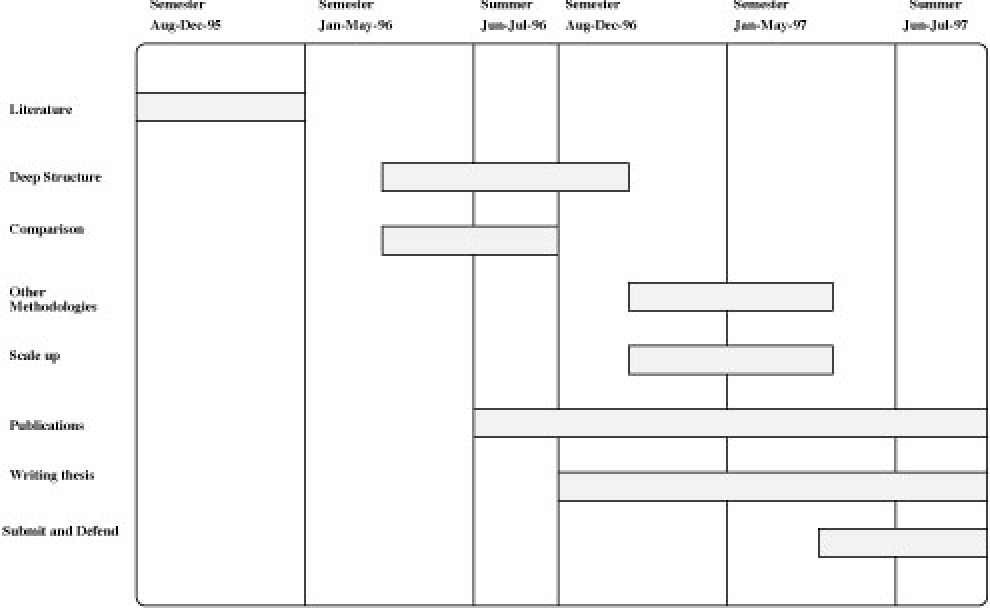
\includegraphics[width=4in,height=3in]{plots/ttphd.pdf}}
	\caption{Cronograma de Actividades para desarrollar la Tesis}
	\label{ttphd}
\end{figure}
\end{comment}
